

% Conclusion
% ------------------------------------------------------------------------------
\setlength{\titleoffset}{0pt}
\section*{Conclusion}

\begin{frame}
  \sectionpage
\end{frame}

\begin{frame}{Contributions}
  \centering
  \vspace{-.3cm}
  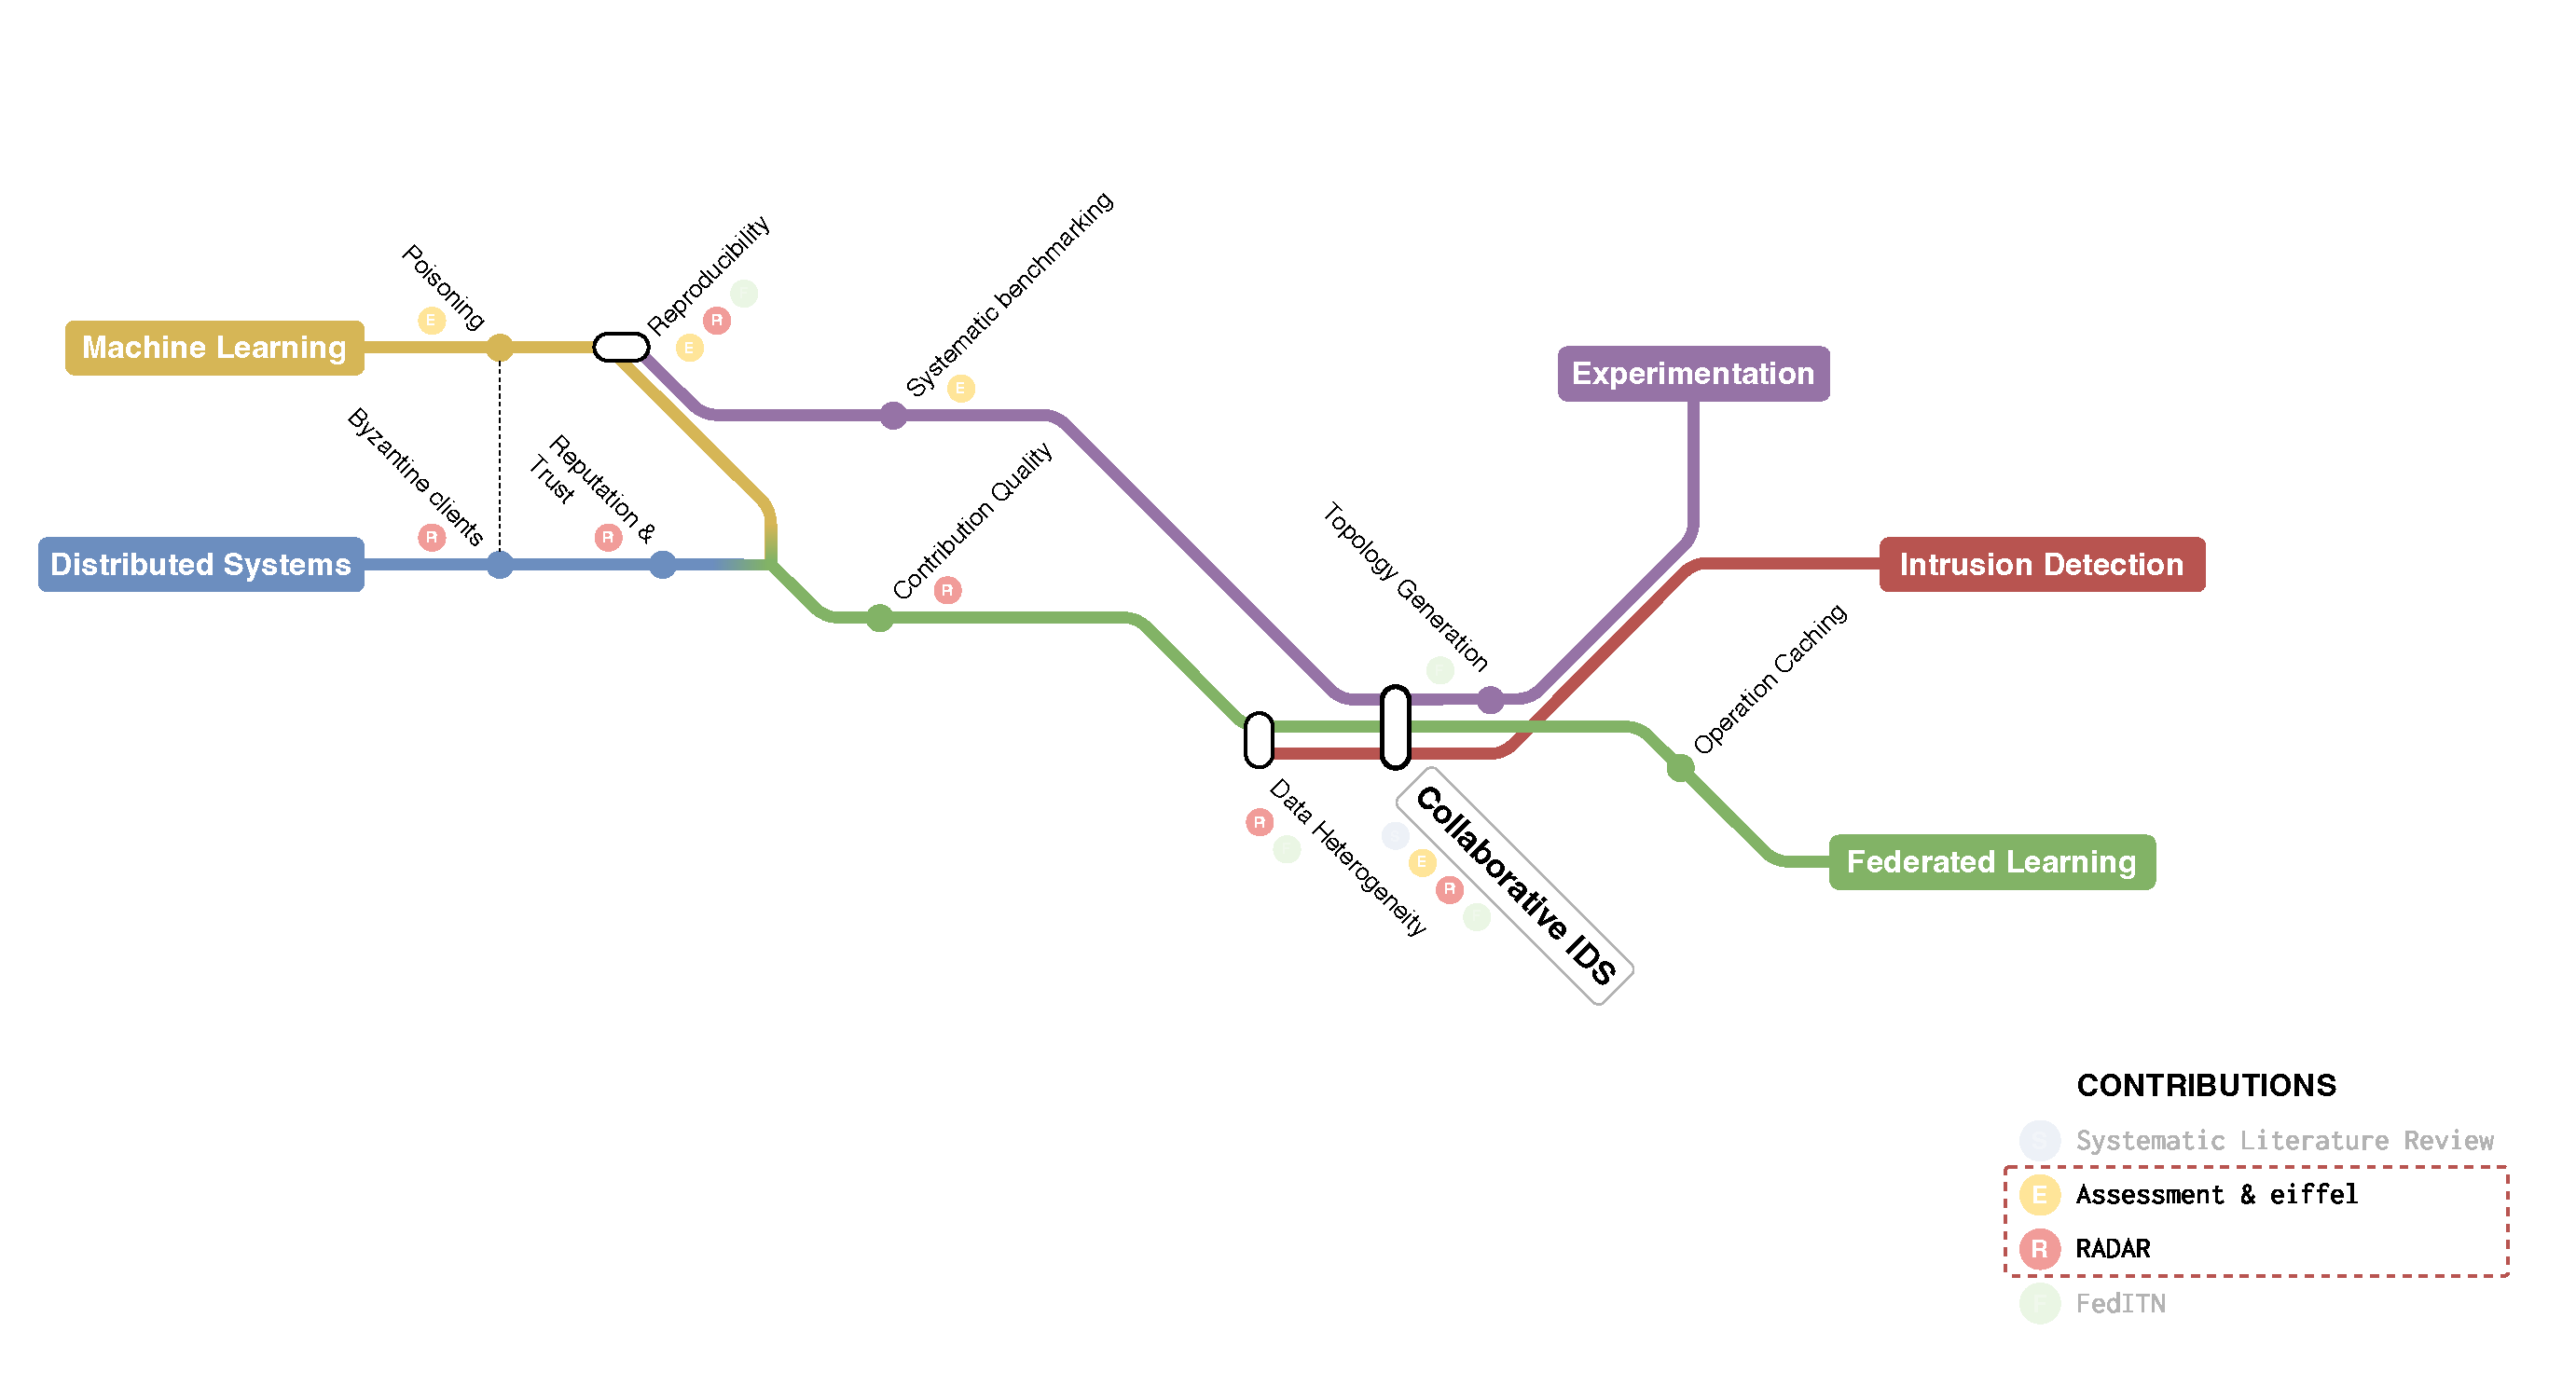
\includegraphics[width=1.1\textwidth, center]{figures/intro/metro/10.pdf}%
  
\end{frame}

% \begin{frame}{Contributions}
%   \textbf{Federated IDSs}
%   \begin{itemize}
%     \item SLR on FIDSs to structure the research field~\autocite{lavaur_tnsm_2022,lavaur_cesar_2022}, with a demonstration of their potential and limitations~\autocite{lavaur_icdcs_demo_2024}
%     \item Assessment of the impact of label-flipping attacks on FIDSs~\autocite{lavaur_ares_bass_2024}, enabled by a reproducible experimental framework
%     \item Countermeasure against Byzantine contributors in FIDSs~\autocite{lavaur_radar_2024}
%   \end{itemize}

%   \onslide<2->{%
%     \textbf{Generating datasets} (the FedITN project)
%     \begin{itemize}
%       \item Constraint-based generation of realistic network topologies (not published yet)
%       \item Generation of realistic network traffic datasets (ongoing work)
%     \end{itemize}
%   }

%   \onslide<3->{%
%     \textbf{Federated Learning}
%     \begin{itemize}
%       \item Feasibility study of operation-caching in FL using Information Centric Networking (ICN)
%       \begin{itemize}
%         \item[$\rightarrow$] Work of Gabriel Bourgeois as part of his Master's internship.
%       \end{itemize}
%     \end{itemize}
%   }
% \end{frame}


% \begin{frame}{Perspectives}
%   \textbf{Four research axes to go beyond FIDSs}
%   \begin{enumerate}
%     \item Modern Detection Techniques
%       \begin{itemize}
%         \item Better representation (\eg, knowledge graphs, embedding, \alert<2>{causality modeling}), explainability, and handling \alert<2>{partial observability}.
%       \end{itemize}
    
%     \item Federated Learning and Derivatives
%       \begin{itemize}
%         \item Handling heterogeneity, trust, decentralization, and going beyond the application layer.
%       \end{itemize}

%     \item Evaluation
%       \begin{itemize}
%         \item More realistic datasets, apt methodologies, and reproducibility.
%       \end{itemize}

%     \item Integration in the Regulatory Landscape
%       \begin{itemize}
%         \item Privacy, data protection, fairness, and compliance with regulations.
%       \end{itemize}

%   \end{enumerate}

% \end{frame}

\begin{frame}[b]{Future Work}
  \centering%
  \vspace{-.3cm}
  \foreach \i in {1,...,4} {%
    \includegraphics<\i>[width=1.1\textwidth, center]{figures/conclusion/future/\i.pdf}%
  }%
\end{frame}


\begin{frame}[b]{Perspectives: Going beyond FIDSs}
  \centering%
  \vspace{-.3cm}
  \foreach \i in {1,...,9} {%
    \includegraphics<\i>[width=1.1\textwidth, center]{figures/conclusion/perspectives/\i.pdf}%
  }%
\end{frame}


\begin{frame}
  \centering
  \scshape\Large Thank you for your attention!

  \vfill
  
  \normalshape\normalsize

  \textbf{Improving Intrusion Detection in Distributed Systems with Federated Learning}
  
  \bigskip
  \raggedright
  \begin{itemize}
    \item Three publications in international \alert{conferences}: ICDCS 2024, ARES (BASS) 2023, and SRDS 2024.
    \item One article in an international \alert{journal}: IEEE TNSM.
    \item National and international \alert{tutorials} on Federated Learning for Intrusion Detection: EUR CyberSchool's Spring Research School 2023, NoF 2023 and ICDCS 2024.
  \end{itemize}

  \vfill
\end{frame}